\documentclass[main.tex]{subfiles}
\begin{document}

\chapter{Energy reconstruction}
\label{chap:energy_reconstruction}
\label{chapter:reconstruction}

This chapter describes the reconstruction chain that connects the station-level measurements of an event to an estimate of the primary cosmic-ray energy.
In \cref{sec:reconstruction_shower_size}, the \Offline reconstruction is used to determine the shower geometry and to estimate the signal at a reference distance from the shower axis through a fit of the \gls{ldf}.
The zenith-angle dependence caused by atmospheric attenuation is then determined and removed in \cref{sec:cic}.
Finally, in \cref{sec:calibration}, the corrected shower size is calibrated against the energy estimator of the \sd{750} to assign an energy to each \sd{433} event.

\section{Reconstruction of the shower size}
\label{sec:reconstruction_shower_size}

The shower reconstruction proceeds in two stages.
First, the relative start times of the signals measured by the participating stations are used to determine the arrival direction of the shower and the impact position of its core on the ground.
The recorded signals are then fitted as a function of the perpendicular distance to the shower axis using an empirical \gls{ldf}.
The value of this function at the reference distance of \SI{300}{\m}, denoted by $S(300)$, provides the ground-level shower-size estimator used for the \sd{433}.
Because the core position affects the station distances entering the \gls{ldf}, the geometry and shower size are finally determined in a combined fit initialized with the results of the separate reconstructions.

\subsection{Geometrical reconstruction}
\label{subsec:geometry_ldf}

The geometrical reconstruction uses the positions and signal start times of the detectors participating in the event.
Its purpose is to determine the position of the shower core on the ground, $\vec{x}_{\mathrm{c}}$, and the unit vector along the shower axis, $\hat{a}$, whose components are the direction cosines from which the zenith angle, $\theta$, and the azimuth angle, $\phi$, are obtained.

The reconstruction begins with a plane-front fit to the station start times, which provides an initial estimate of the arrival direction.
The signal-weighted barycentre of the participating stations is used as the initial estimate of the core position.
These estimates are subsequently refined using a curved description of the shower front.

In the \Offline reconstruction, the extreme shower front is approximated by a sphere expanding at the speed of light from a virtual origin $\vec{x}_0$ at time $t_0$.
The predicted time at which this front reaches a position $\vec{x}$ is
\begin{align}
    c\,t_\mathrm{sh}(\vec{x}) = c\,t_0 + \lvert \vec{x}-\vec{x}_0 \rvert .
    \label{eq:spherical_shower_front}
\end{align}
The fit minimizes the squared differences between the measured and predicted start times,
\begin{align}
    \chi^2 = \sum_i \frac{\left[t_i-t_\mathrm{sh}(\vec{x}_i)\right]^2}{\sigma_{t_i}^2}.
    \label{eq:geometry_chi2}
\end{align}
where $t_i$ and $\sigma_{t_i}$ are the start time measured by station $i$ and its uncertainty, respectively.

The core position is refined together with the lateral distribution of the station signals.
Once $\vec{x}_{\mathrm{c}}$ is determined, the reconstructed shower direction is given by
\begin{align}
    \hat{a}
    =
    \frac{\vec{x}_{0}-\vec{x}_{\mathrm{c}}}
    {\left|\vec{x}_{0}-\vec{x}_{\mathrm{c}}\right|}.
    \label{eq:shower_axis}
\end{align}
The radius of curvature at the core position is
\begin{align}
    R_{0}=\left|\vec{x}_{0}-\vec{x}_{\mathrm{c}}\right|.
\end{align}

For events with at least five participating stations, the radius of curvature is determined from the timing fit.
For events with lower station multiplicity, the number of degrees of freedom is insufficient to constrain the curvature, and $R_{0}$ is fixed according to a parametrization obtained from higher-multiplicity events.

The left panel of \cref{fig:sd433_event_footprint_ldf} illustrates the geometrical reconstruction of an \sd{433} event.
The marker size is proportional to the station signal, while the colour scale represents its start time, progressing from earlier signals in blue to later signals in green.
The black line indicates the reconstructed arrival direction projected onto the ground, and the cross marks the reconstructed core position.
% TODO: Describe the Offline geometrical reconstruction and the modified NKG
% lateral-distribution function used for SD-433, including the fixed beta
% parametrization and the definition of S(300).

\begin{figure}[t]
    \centering
    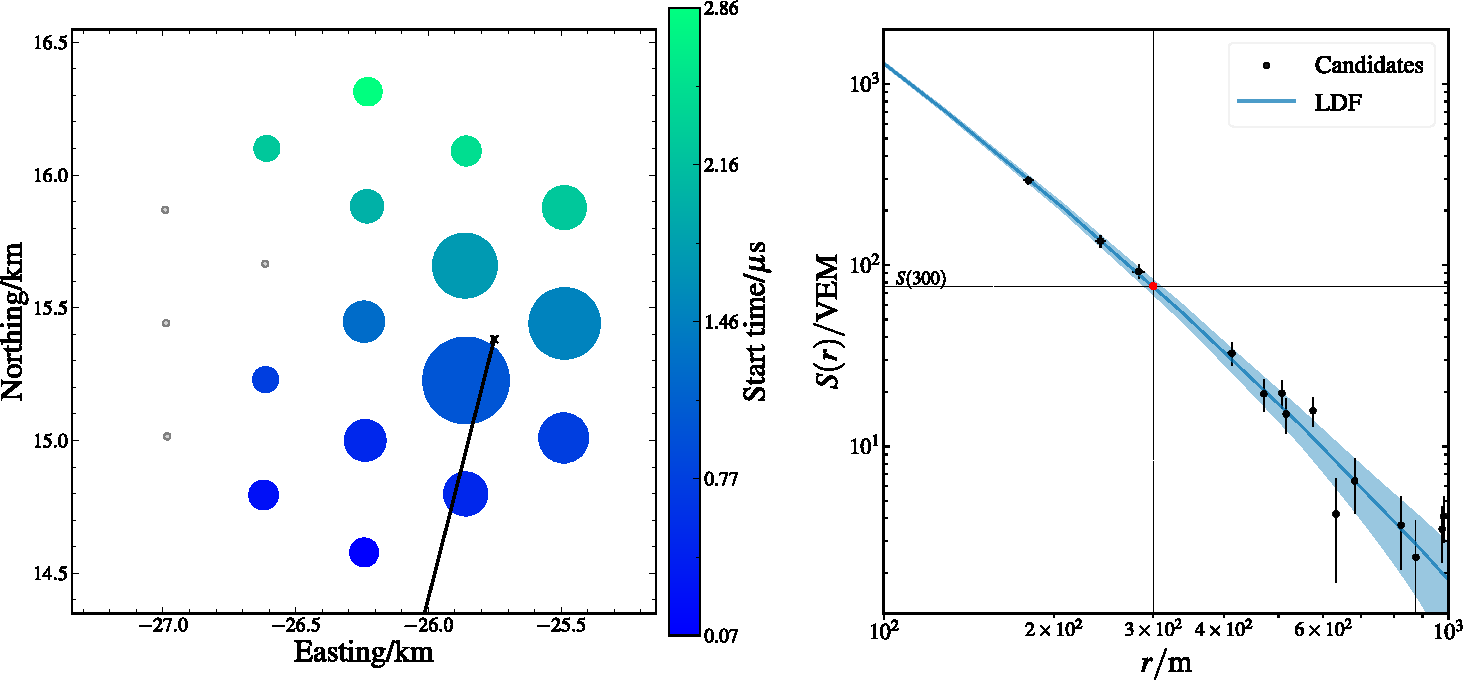
\includegraphics[width=\textwidth]{figures/chapter_reconstruction/event_footprint_ldf.pdf}
    \caption{Example SD-433 event reconstruction. The left panel shows the event footprint, with marker size proportional to the recorded signal $S(r)$ and colour indicating the station start time. The right panel shows the decrease of the signal with distance $r$ from the shower axis and the \gls{ldf} fit using a modified \gls{nkg} function. The red point marks the reconstructed shower-size estimator $S(300)$.}
    \label{fig:sd433_event_footprint_ldf}
\end{figure}

\subsection{Properties of the reconstructed sample}
\label{subsec:reconstructed_sample}

% TODO: Introduce the complete reconstructed sample before the later quality,
% zenith, CIC, and calibration selections. State the S(300) >= 0.1 VEM display
% threshold and the 0--60 degree zenith range used in these distributions.

\begin{figure}[t]
    \centering
    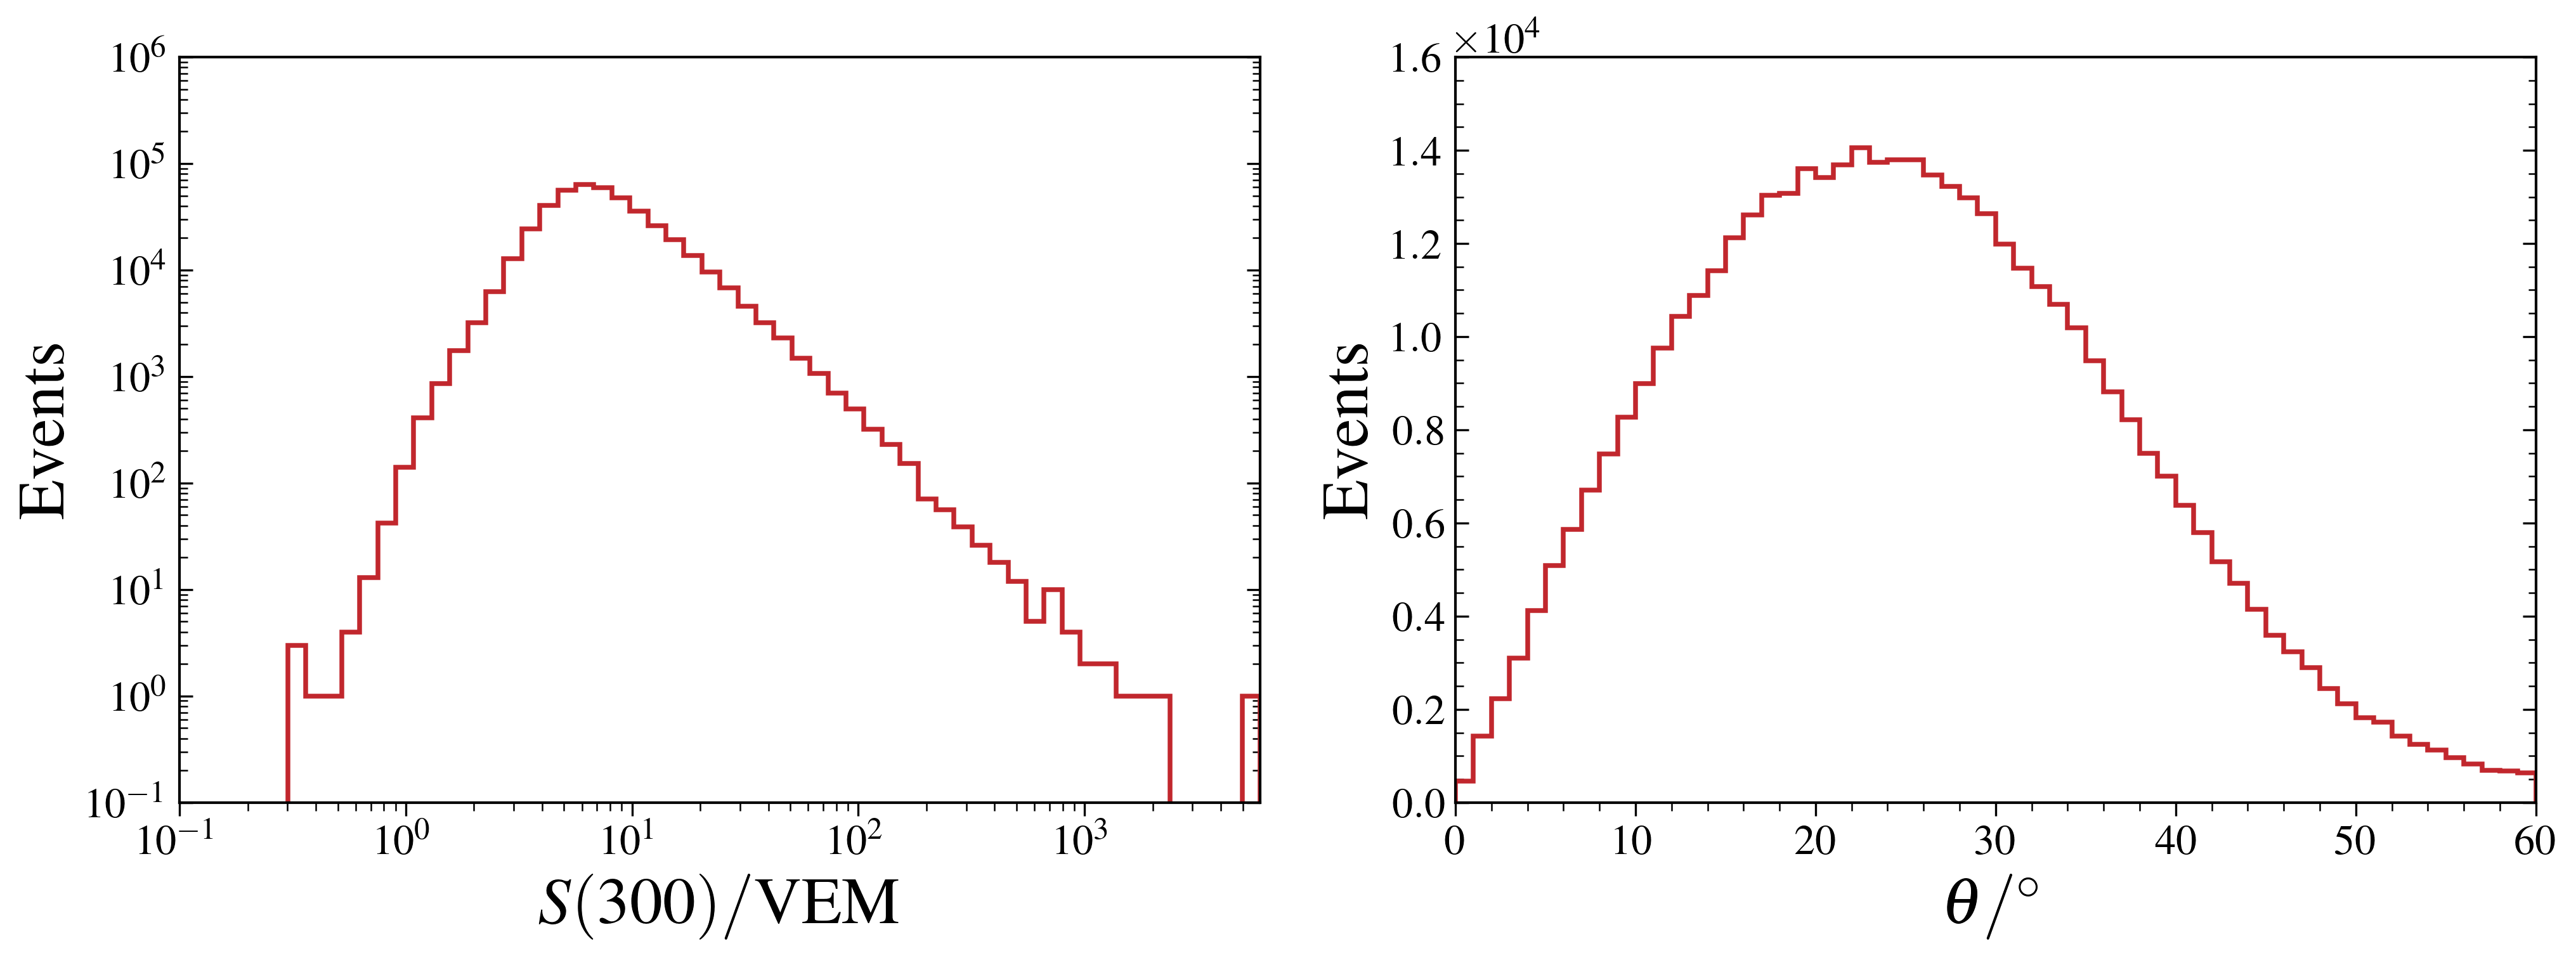
\includegraphics[width=\textwidth]{figures/chapter_reconstruction/shower_size_zenith_distributions.png}
    \caption{Distributions of the reconstructed shower size $S(300)$ (left) and zenith angle (right) for SD-433 events with $S(300)\geq0.1\,\mathrm{VEM}$ and $0^\circ\leq\theta<60^\circ$, before the subsequent analysis selections.}
    \label{fig:sd433_size_zenith_distributions}
\end{figure}

\begin{figure}[t]
    \centering
    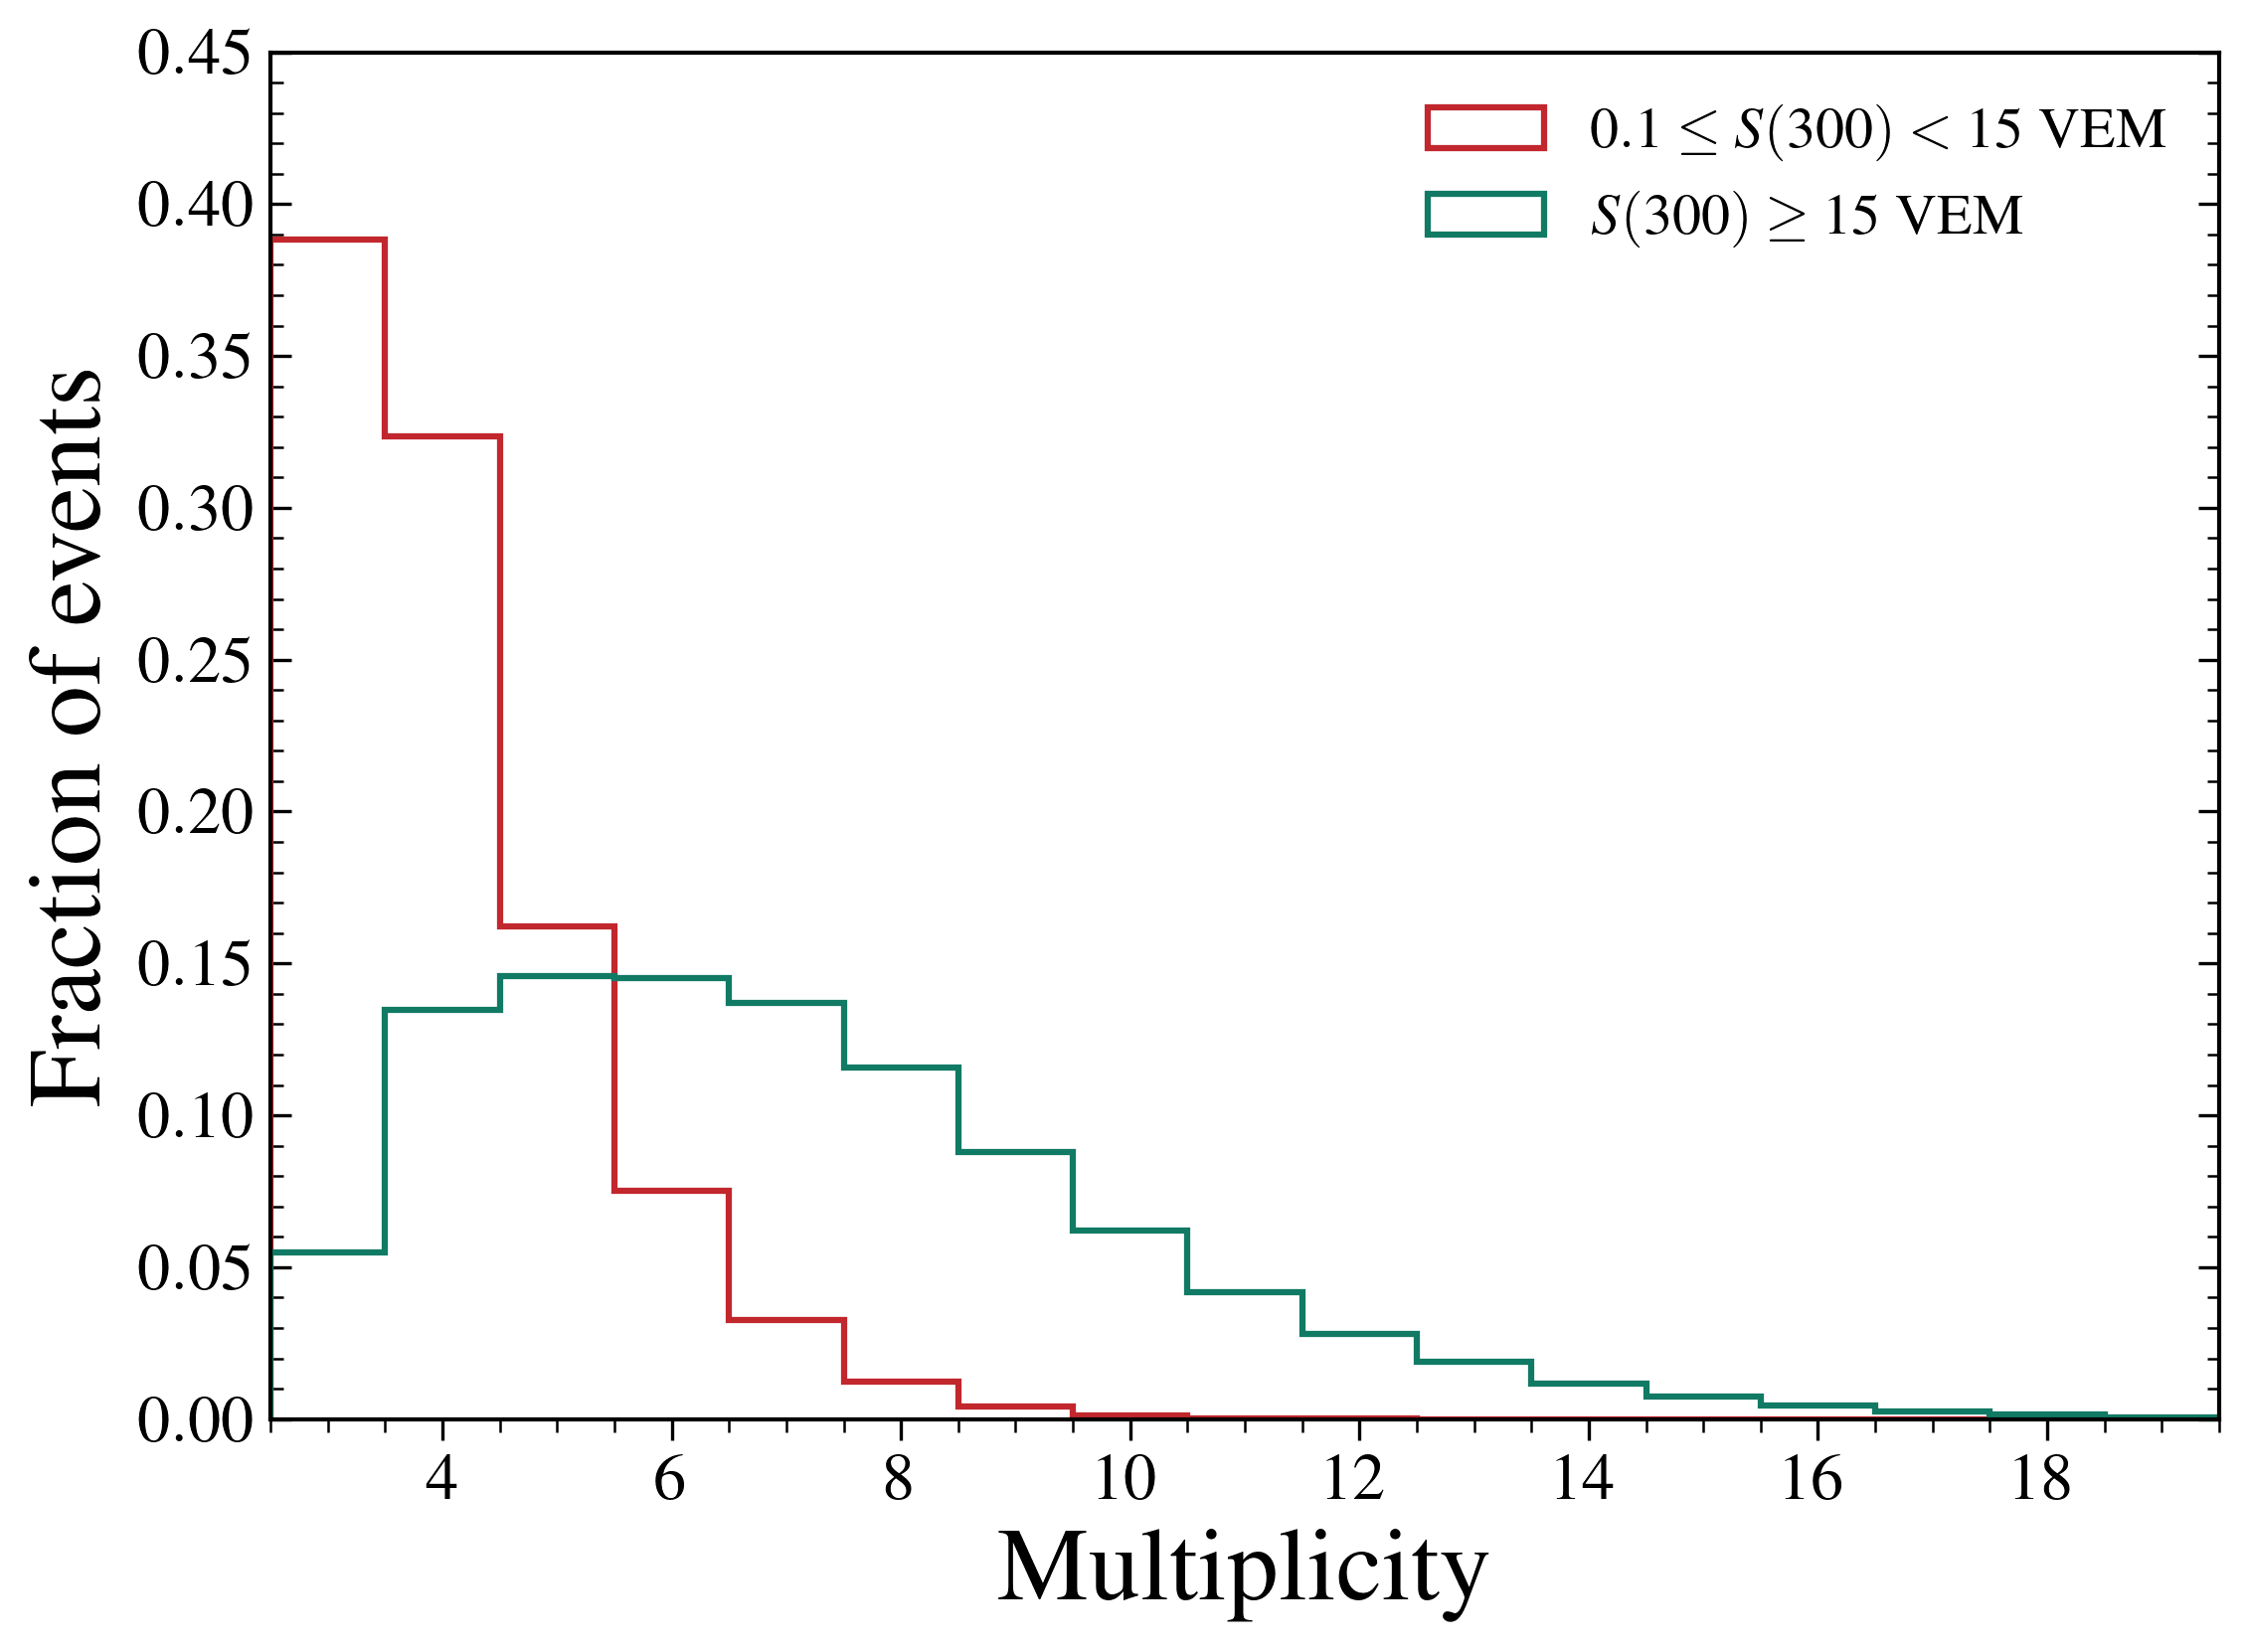
\includegraphics[width=0.78\textwidth]{figures/chapter_reconstruction/multiplicity_by_shower_size.png}
    \caption{Selected-station multiplicity for reconstructed events below and above $S(300)=15\,\mathrm{VEM}$. Each distribution is normalized independently to show the change in its shape with shower size.}
    \label{fig:sd433_multiplicity}
\end{figure}

\section{Correction for zenith-angle attenuation}
\label{sec:cic}

\subsection{Constant-intensity cuts}
\label{subsec:cic_method}

% TODO: Explain the constant-intensity or countdown construction, the use of
% nine equal-exposure bins in sin^2(theta), the six event intensities, the
% 30-degree reference angle, and the extension of the CIC fit to 45 degrees.

\begin{figure}[t]
    \centering
    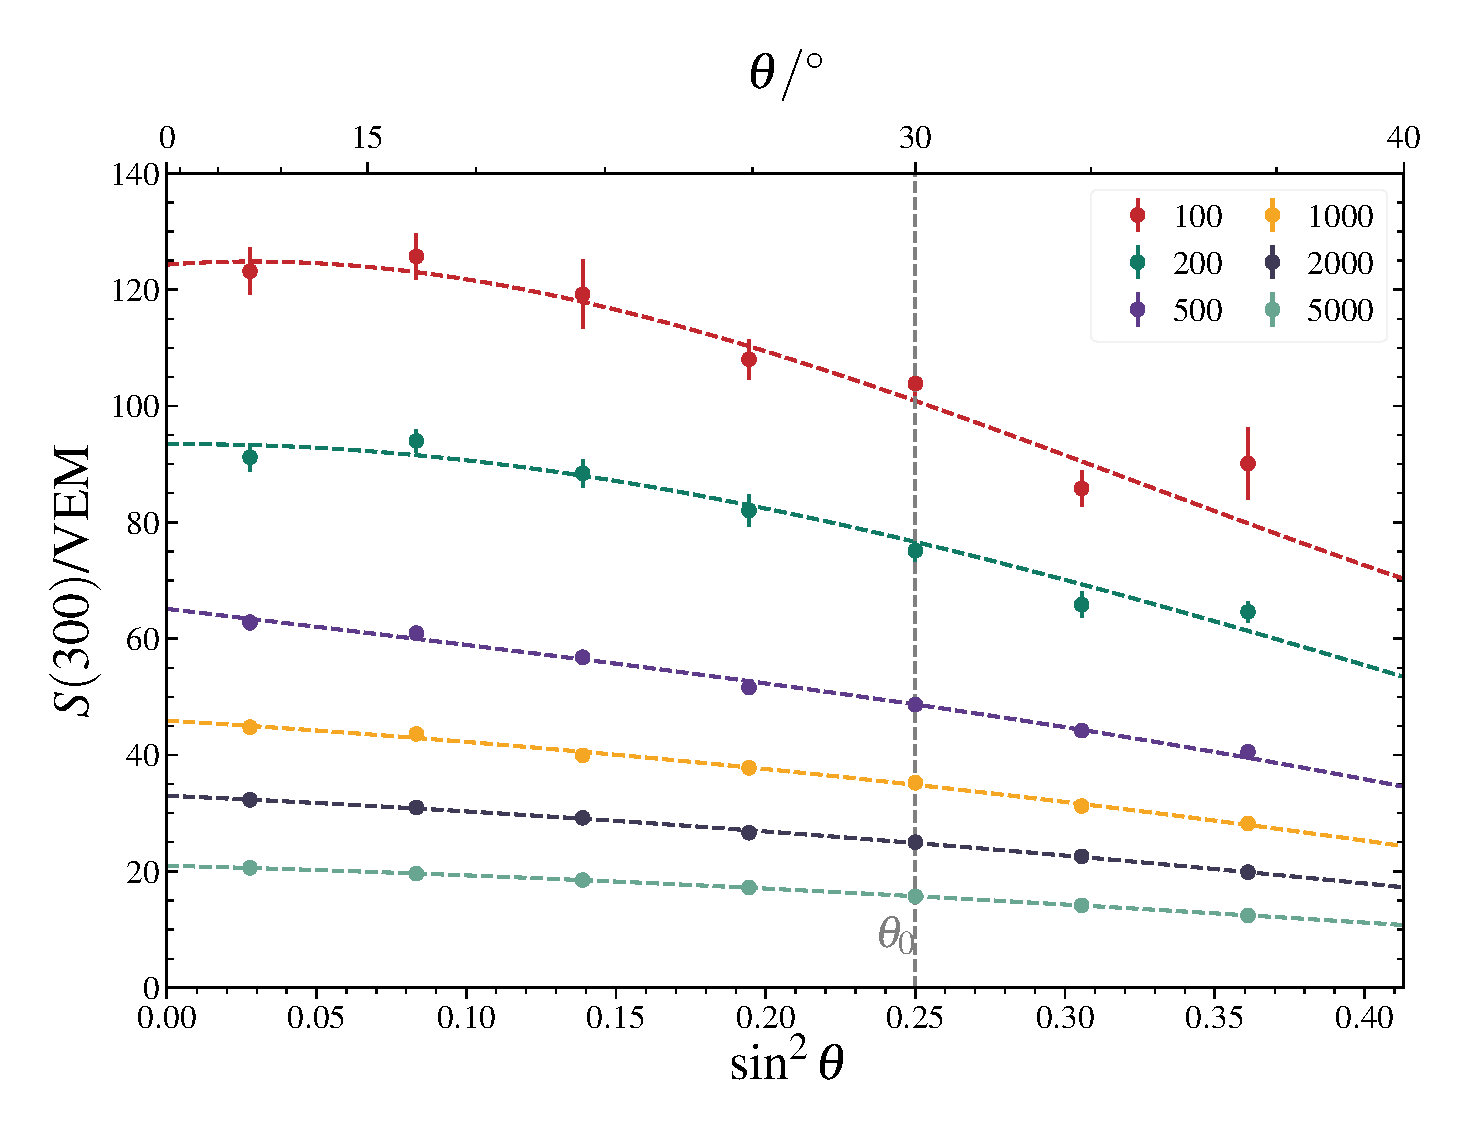
\includegraphics[width=0.85\textwidth]{figures/chapter_reconstruction/cic_individual_cuts.pdf}
    \caption{Independent fits to the six constant-intensity cuts used to determine the zenith-angle attenuation of $S(300)$.}
    \label{fig:cic_individual_cuts}
\end{figure}

\subsection{Energy-dependent attenuation model}
\label{subsec:cic_global_model}

% TODO: Motivate the energy-dependent CIC parametrization, following the
% established SD reconstruction approach, and report the fitted coefficients
% and their uncertainties in both the Spectuls and Offline conventions.

\begin{figure}[t]
    \centering
    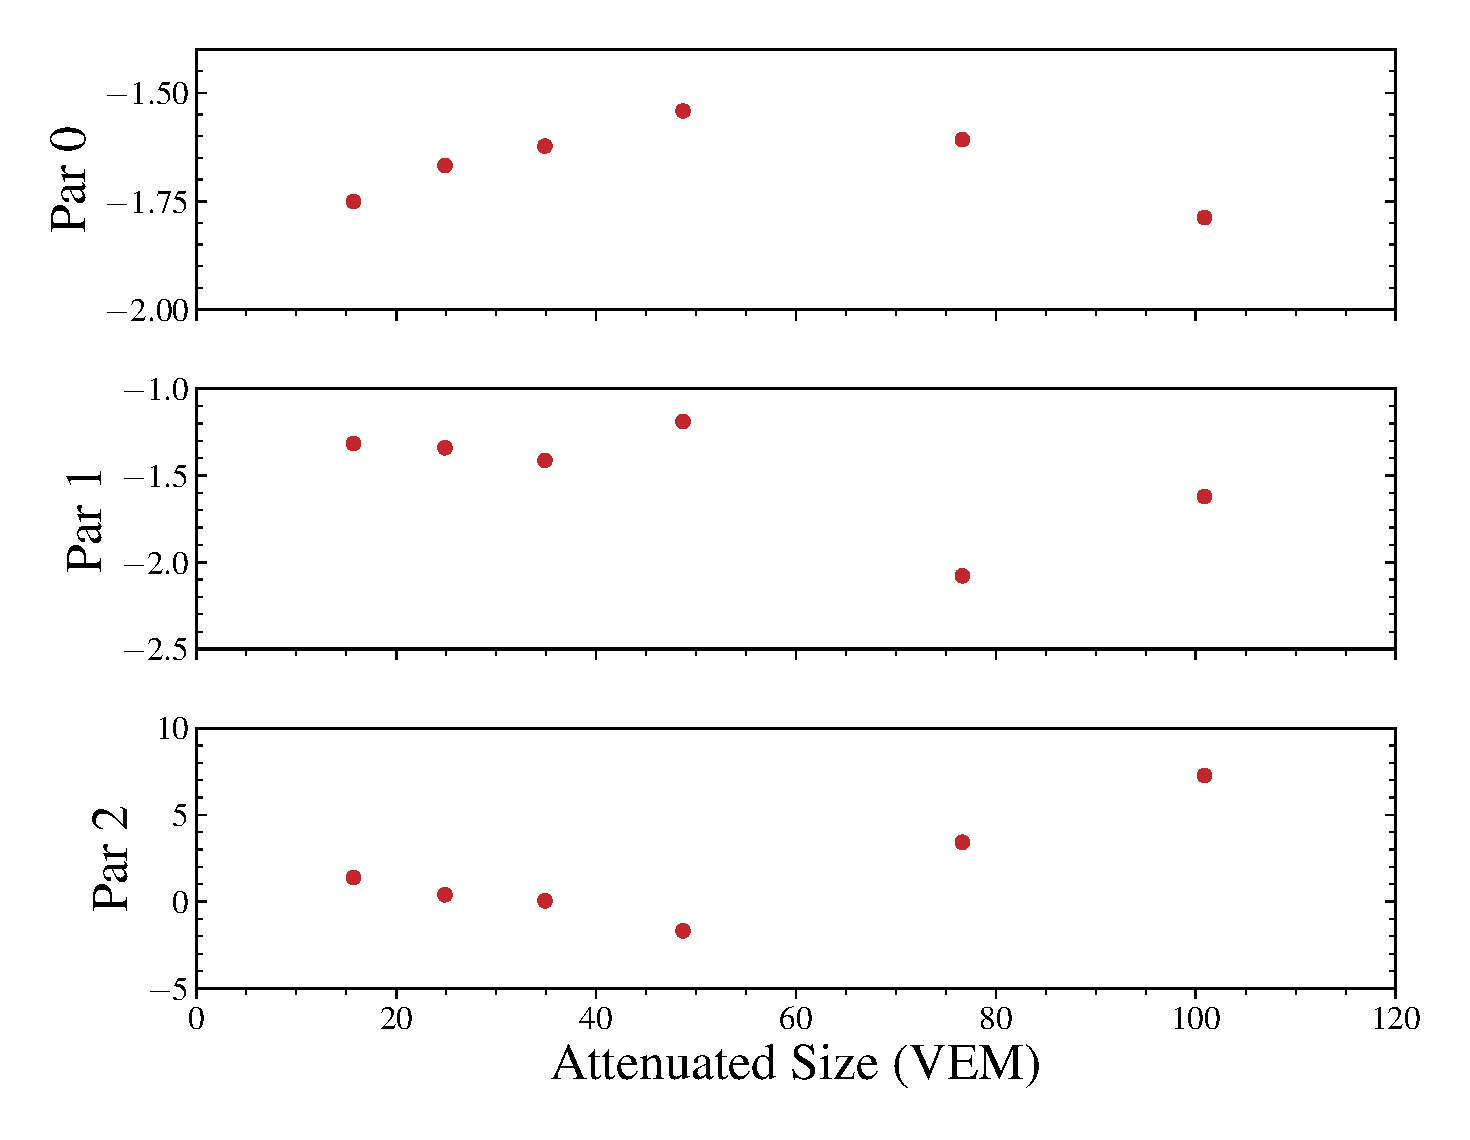
\includegraphics[width=0.85\textwidth]{figures/chapter_reconstruction/cic_individual_parameters.pdf}
    \caption{Evolution of the attenuation-curve parameters obtained from the independent constant-intensity fits. This dependence motivates the global shower-size-dependent CIC model.}
    \label{fig:cic_individual_parameters}
\end{figure}

\begin{figure}[t]
    \centering
    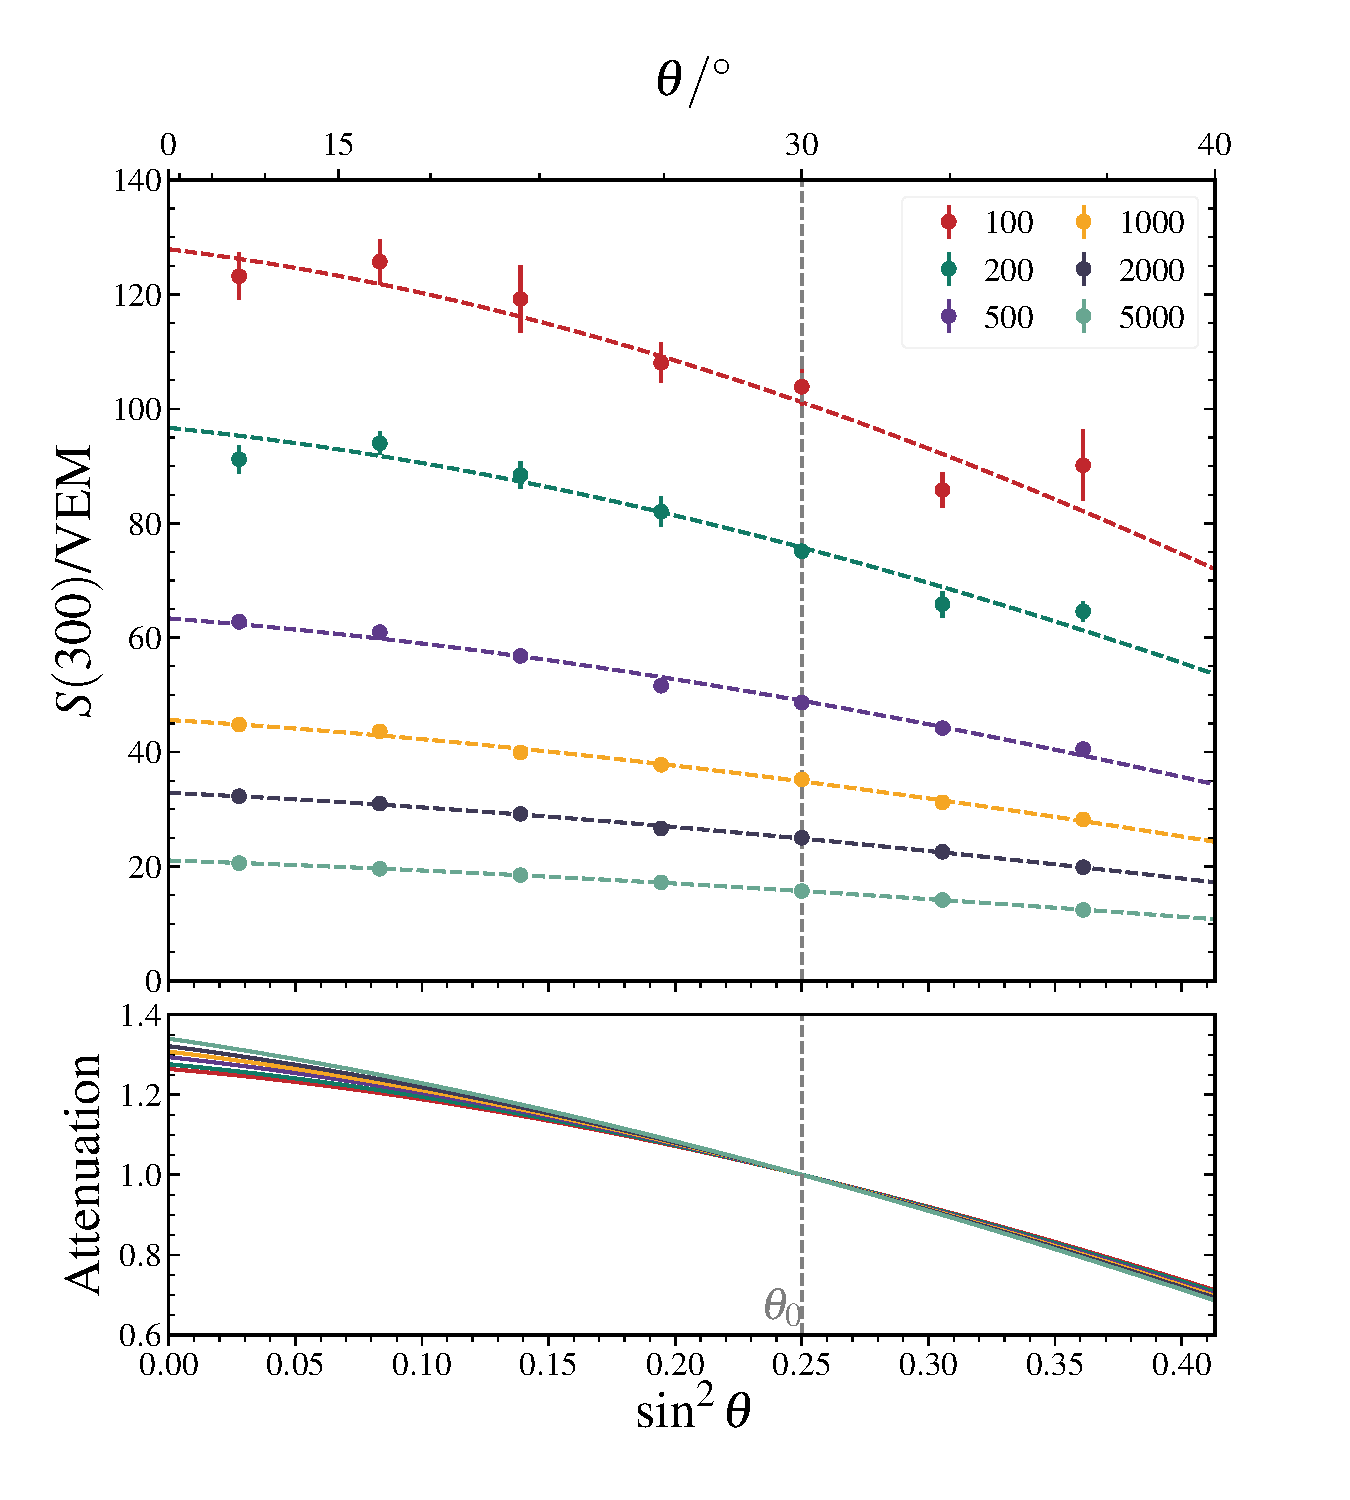
\includegraphics[width=0.85\textwidth]{figures/chapter_reconstruction/cic_global_fit.pdf}
    \caption{Global energy-dependent fit to the SD-433 constant-intensity cuts.}
    \label{fig:cic_global_fit}
\end{figure}

\begin{figure}[t]
    \centering
    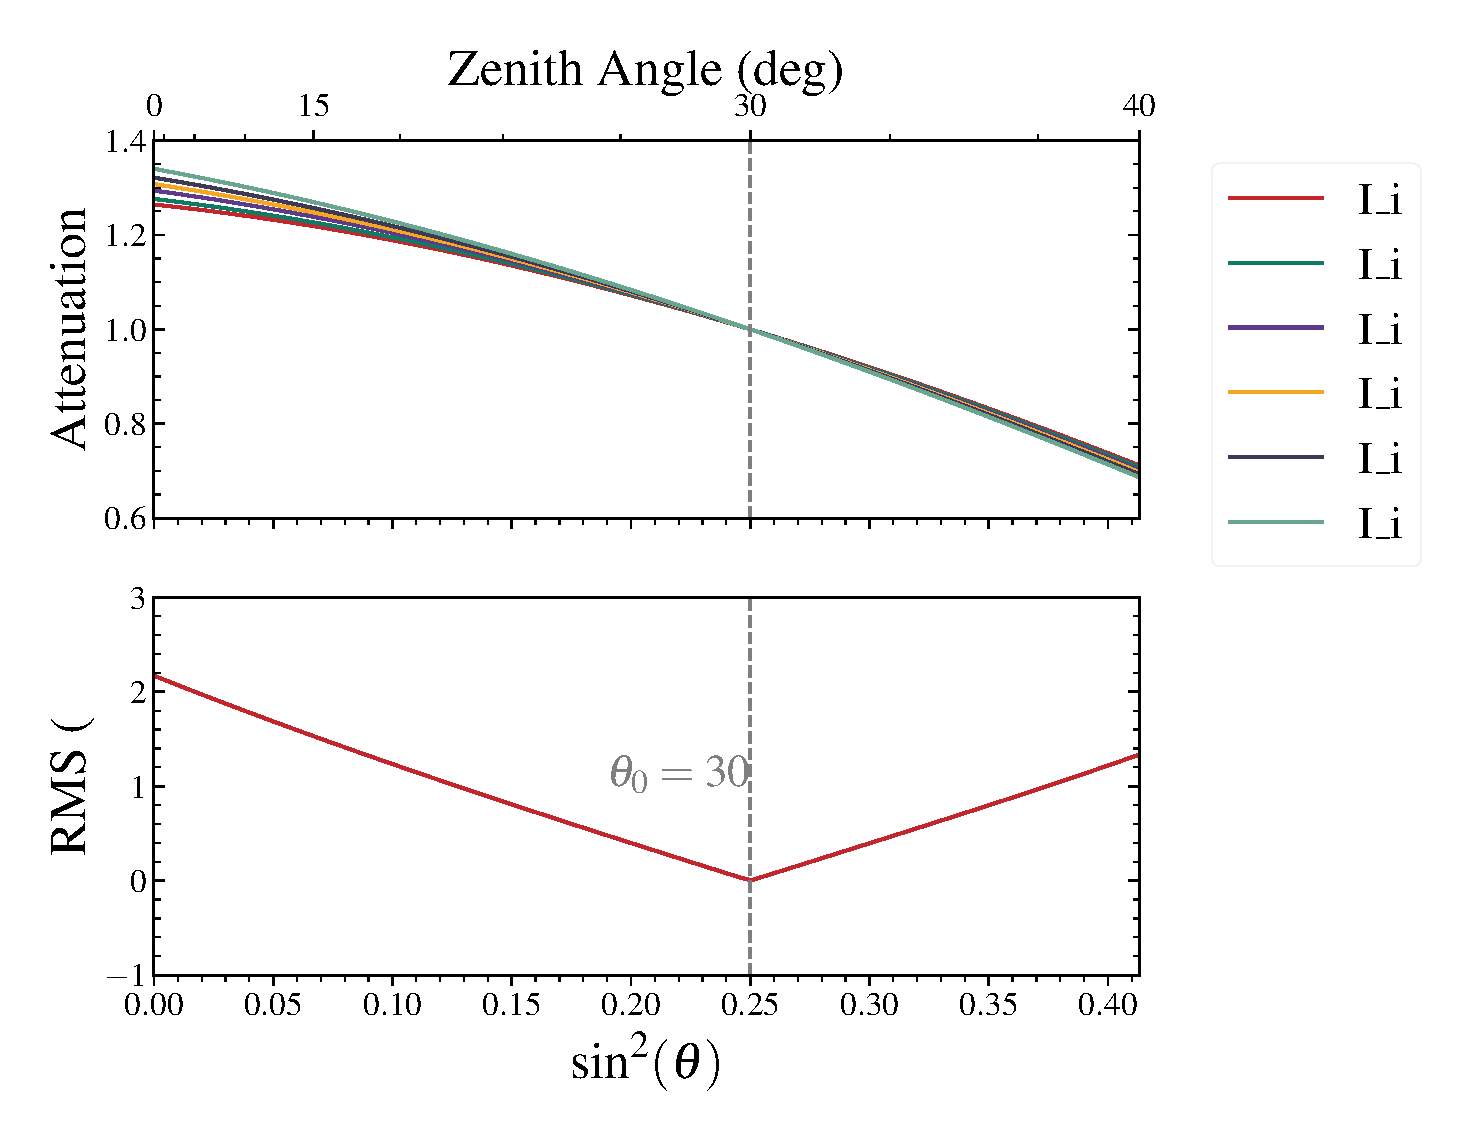
\includegraphics[width=0.85\textwidth]{figures/chapter_reconstruction/cic_attenuation.pdf}
    \caption{Attenuation curves obtained from the global CIC fit for the shower sizes sampled by the constant-intensity cuts. The curves define the conversion from $S(300)$ to the reference estimator $S_{30}$.}
    \label{fig:cic_attenuation}
\end{figure}

\subsection{Fit quality and CIC-corrected estimator}
\label{subsec:cic_validation}

% TODO: Report chi2/ndf = 31.80/43, p = 0.8959, discuss the residuals,
% and define the event-by-event conversion from S(300) to S30.

\begin{figure}[t]
    \centering
    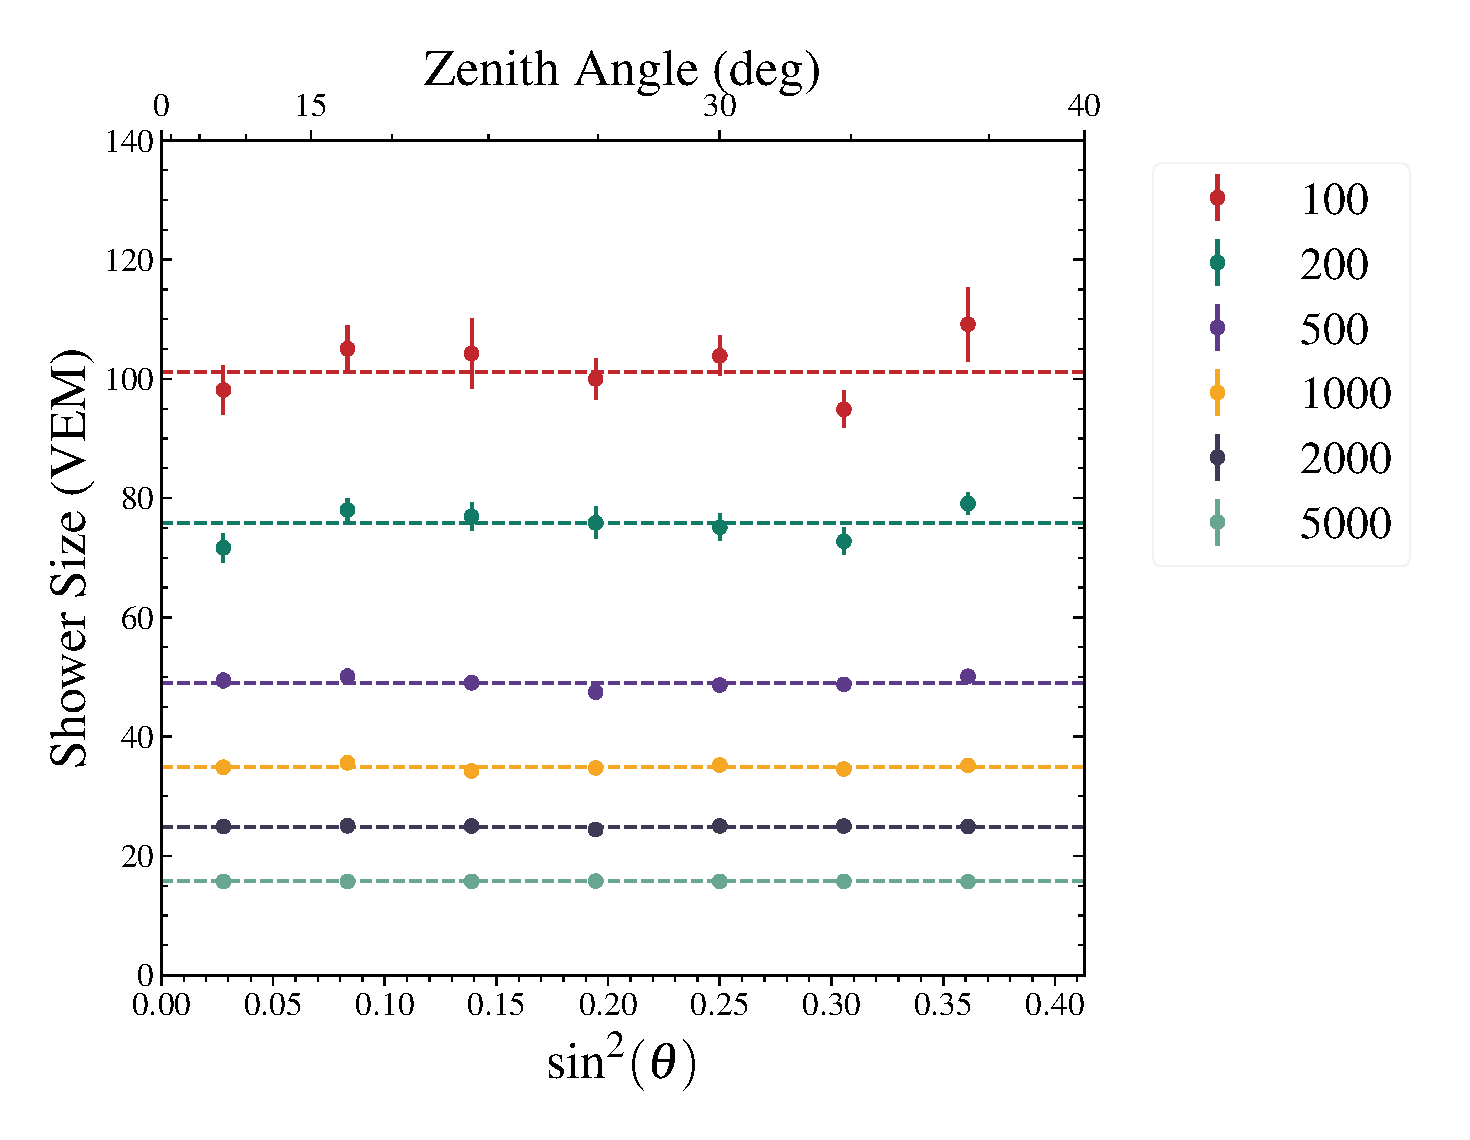
\includegraphics[width=0.85\textwidth]{figures/chapter_reconstruction/cic_residuals.pdf}
    \caption{Residuals of the global CIC fit for the six constant-intensity cuts.}
    \label{fig:cic_residuals}
\end{figure}

\section{Calibration of the SD-433 energy estimator}
\label{sec:energy_calibration}
\label{sec:calibration}

\subsection{SD-750 reference scale and coincident events}
\label{subsec:calibration_sample}

% TODO: Describe the SD-750 reference energy scale, the construction of the
% 37,505-event coincidence sample, the resolution model, and the S30 > 30 VEM
% calibration threshold that leaves 5,980 events for the fit.

\subsection{Likelihood fit and calibration relation}
\label{subsec:calibration_fit}

% TODO: Introduce E = A (S30 / 40 VEM)^B, describe the preliminary chi-square
% fit and the final likelihood treatment, and report A, B, their scaled
% uncertainties, and their correlation.

\begin{figure}[t]
    \centering
    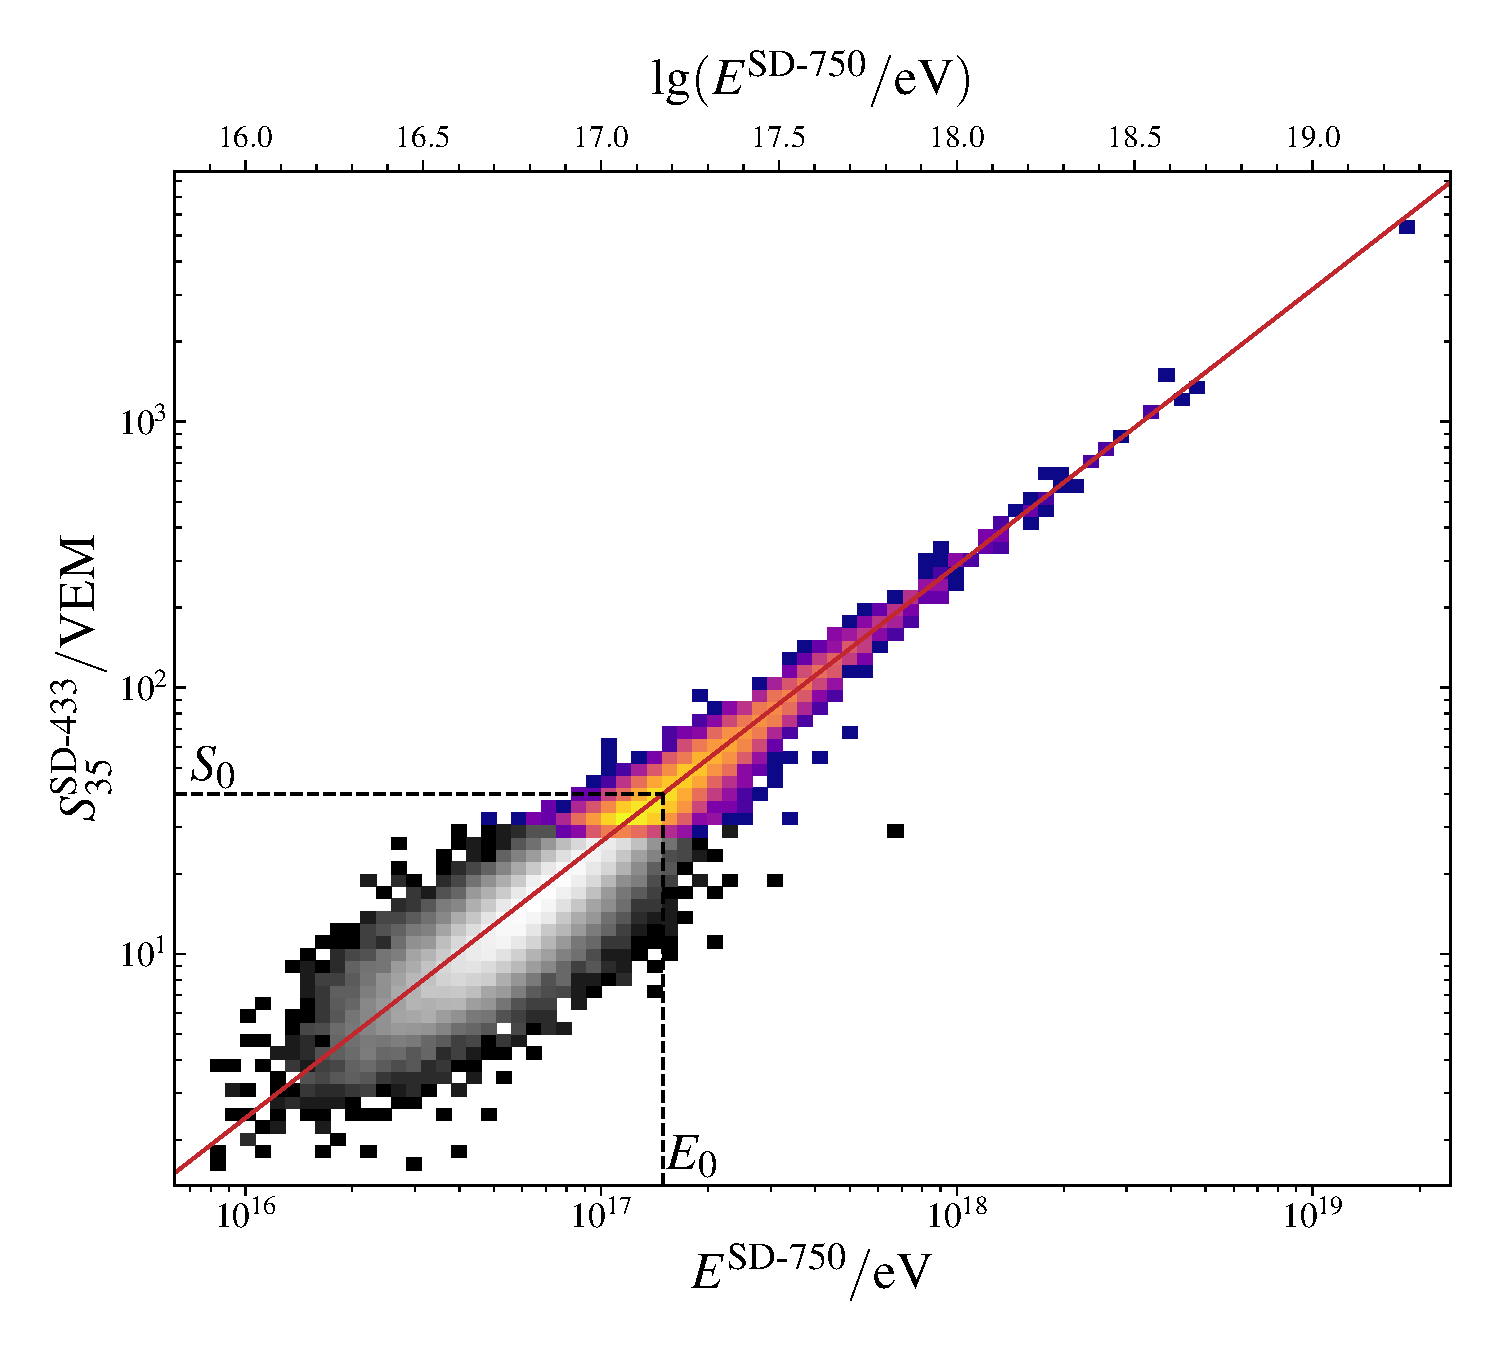
\includegraphics[width=0.82\textwidth]{figures/chapter_reconstruction/energy_calibration.pdf}
    \caption{Calibration of the SD-433 zenith-corrected shower size $S_{30}$ against the SD-750 reference energy using coincident events. The line shows the fitted power-law relation.}
    \label{fig:sd433_energy_calibration}
\end{figure}

\subsection{Calibration residuals and application}
\label{subsec:calibration_validation}

% TODO: Discuss the calibration residuals, the 113.3 PeV energy associated
% with the 30 VEM calibration cut, and application of the relation to the
% 382,131-event SD-433 dataset used for the spectrum measurement.

\begin{figure}[t]
    \centering
    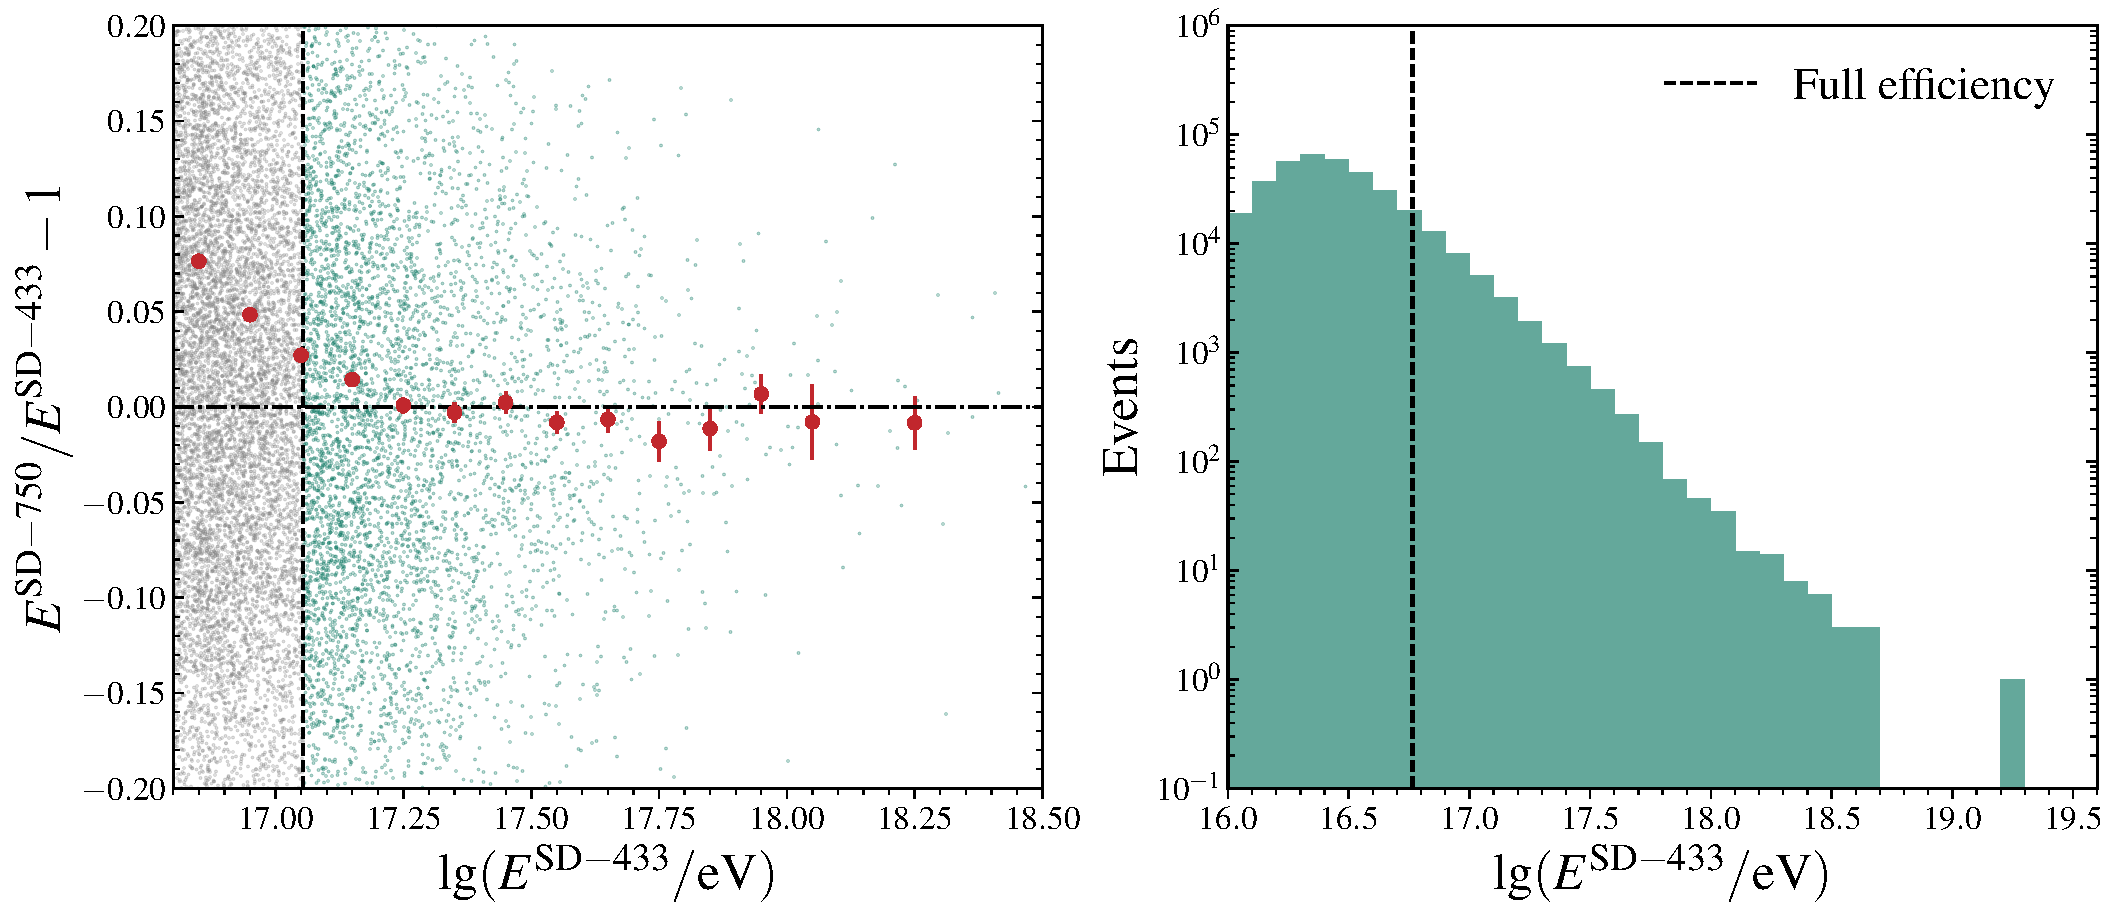
\includegraphics[width=0.82\textwidth]{figures/chapter_reconstruction/energy_calibration_residuals.pdf}
    \caption{Residuals of the SD-433 energy-calibration fit.}
    \label{fig:sd433_energy_calibration_residuals}
\end{figure}

\section{Summary}
\label{sec:energy_reconstruction_summary}

% TODO: Summarize the continuous reconstruction chain from the Offline
% determination of S(300), through the CIC correction to S30, to the calibrated
% SD-433 energy used in the spectrum measurement.

\end{document}
